\subsection{Menambahkan skematik baru}

Skematik baru dapat ditambahkan ke dalam project dengan memilih menu
{\sf File $\rightarrow$ New}. Pilih {\sf New Diagram/Schematic File}, kemudian
{\sf OK}.

\begin{figure}[H]
\centering
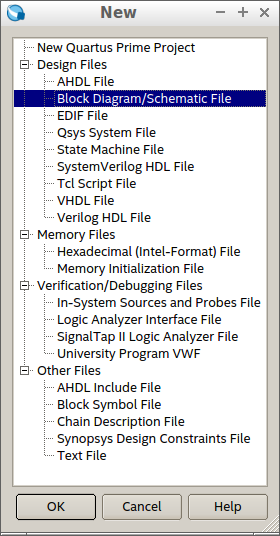
\includegraphics[scale=0.5]{images/NewSchematic.png}
\par
\end{figure}

File skematik kosong akan terbuka pada tab baru dengan nama {\sf Block1.bdf}.
Kita dapat membuat skematik yang kita inginkan pada file ini.

\begin{figure}[H]
\centering
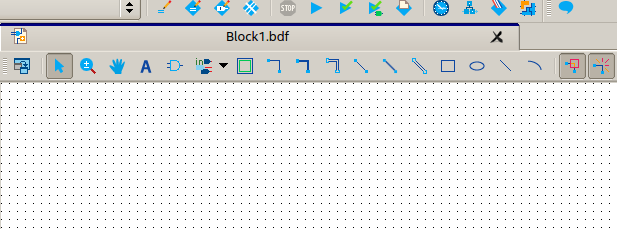
\includegraphics[scale=0.5]{images/EmptySchematic.png}
\par
\end{figure}

Untuk menambahkan komponen, dapat dilakukan dengan cara mengklik toolbar
{\sf Symbol Tool}.

\begin{figure}[H]
\centering
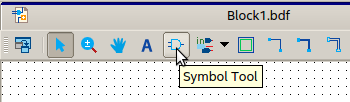
\includegraphics[scale=0.5]{images/SymbolTool.png}
\par
\end{figure}

Komponen yang ingin ditambahkan pada skematik dapat diperoleh dengan
ekspasi node {\sf Libraries}, mencari komponen tersebut, dan memilihnya.
Misalkan kita ingin menambahkan gerbang AND dengan dua input, maka dapat dipilih
pada {\sf primitives $\rightarrow$ logic $\rightarrow$ and2}. Klik
{\sf OK} setelah komponen yang diinginkan telah dipilih.

\begin{figure}[H]
\centering
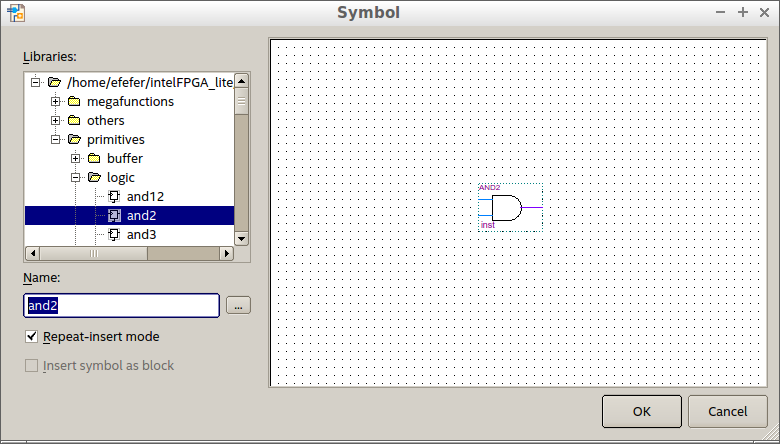
\includegraphics[scale=0.5]{images/BlockAnd.png}
\par
\end{figure}

Pemilihan komponen juga dapat dilakukan dengan mengetikkan nama komponen yang
diinginakan pada isian {\sf Name}, misalnya {\sf jkff} untuk J-K flip-flop.

Khusus untuk menambahkan komponen input dan output, dapat juga digunakan
toolbar {\sf Pin Tool}.
\begin{figure}[H]
\centering
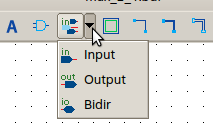
\includegraphics[scale=0.5]{images/PinTool.png}
\par
\end{figure}

Untuk menghubungkan antara satu komponen dengan komponen yang lain, dapat
digunakan {\sf Orthogonal Node Tool}.
\begin{figure}[H]
\centering
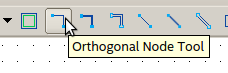
\includegraphics[scale=0.5]{images/OrthogonalNodeTool.png}
\par
\end{figure}

Berikut ini adalah contoh skematik untuk multiplexer 2-to-1:
\begin{figure}[H]
\centering
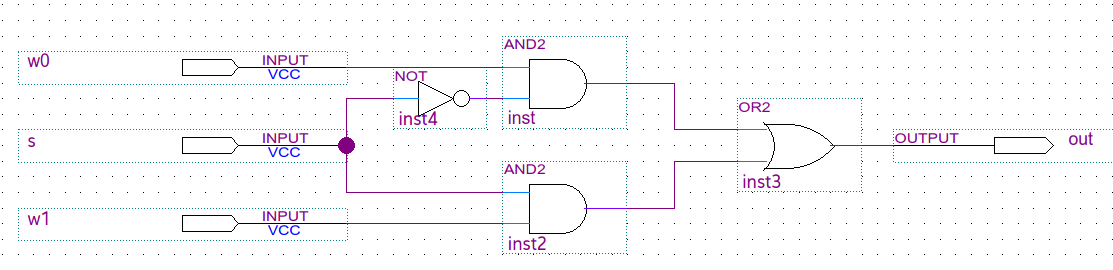
\includegraphics[width=\textwidth]{images/sch_mux_2_1.png}
\par
\end{figure}

Skematik ini kemudian dapat digunakan untuk proses lebih lanjut seperti
simulasi dan download ke hardware FPGA.
